\documentclass{plt}
\usepackage{bbding} % \Checkmark \XsolidBold
\usetheme{metropolis}           % Use metropolis theme

\title{Programming Languages and Translators}
\author{Ronghui Gu}
\institute{Columbia University}
\date{Spring 2019}
%\titlegraphic{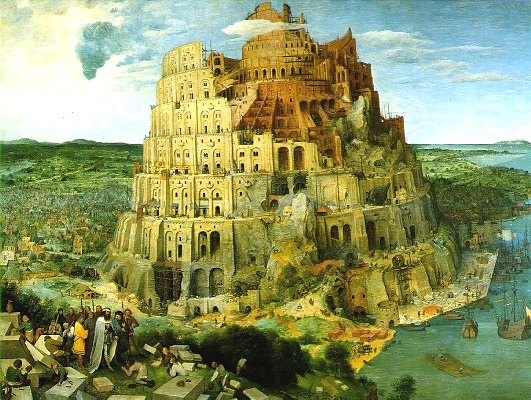
\includegraphics[width=0.35\textwidth]{bruegel-tower-of-babel.jpg}
%{\tiny Pieter Bruegel, \emph{The Tower of Babel}, 1563}
%}


\newenvironment{rightpopup}{
\begin{lrbox}{\shadowblockbox}%
\begin{beamercolorbox}[rounded=true,shadow=true,wd={0.6\textwidth},sep=0pt,leftskip=3pt]{popup}}{\end{beamercolorbox}
\end{lrbox}
\hbox{\hskip0.45\textwidth\vbox to 0pt{\vss\only<2>{\usebox{\shadowblockbox}}\vskip13pt}}%
\vskip-\baselineskip
}

\newenvironment{leftpopup}{
\begin{lrbox}{\shadowblockbox}%
\begin{beamercolorbox}[rounded=true,shadow=true,wd={0.5\textwidth},sep=0pt,leftskip=3pt]{popup}}{\end{beamercolorbox}
\end{lrbox}%
\noindent
\hbox{\vbox to 0pt{\vss\only<2>{\usebox{\shadowblockbox}}}}%
}



\begin{document}

\frame{\titlepage}

\begin{frame}{Instructor}

\parskip=0.3\baselineskip

Prof. \href{http://guronghui.com}{\textcolor{mBlue}{Ronghui Gu}}

515 Computer Science Building

\email{ronghui.gu@columbia.edu}

%\url{http://guronghui.com}

Office hours: Thursdays 1:30 - 2:30 PM / by appointment

\vfill


\vfill
\small{Prof. Stephen A. Edwards and Prof. Baishakhi Rey also teach 4115.}
\small{$^*$These slides are borrowed from Prof. Edwards.}

\end{frame}

\begin{frame}[fragile]{What is a Programming Language?}

A programming language is a notation that  a person and a computer can both understand.
\begin{itemize}

\item It allows you to express what is the \textbf{task} to compute

\item It allows a computer to \textbf{execute} the computation task

\end{itemize}


Every  programming language has a \textbf{syntax} and \textbf{semantics}.
\begin{itemize}

\item Syntax: how characters combine to form a program

\item Semantics: what the program \emph{means}

\end{itemize}

\end{frame}


\begin{frame}[fragile]{Components of a language: Syntax}

\alert{How characters combine to form a program.}

\begin{quote}
Calculate the n-th Fibonacci number.
\end{quote}

is syntactically correct English, but isn't a Java program.

\begin{java}
class Foo {
  public int j;
  public int foo(int k) { return j + k; }
}
\end{java}

is syntactically correct Java, but isn't C.

\end{frame}

\begin{frame}{Specifying Syntax}

Usually done with a \alert{context-free grammar}.

Typical syntax for algebraic expressions:

\[
\begin{array}{rcl}
\textit{expr} & \rightarrow & \textit{expr} + \textit{expr} \\
& | &  \textit{expr}\ -\ \textit{expr} \\
& | &  \textit{expr}\ *\ \textit{expr} \\
& | &  \textit{expr}\ /\ \textit{expr} \\
& | &  (\ \textit{expr}\ ) \\
& | &  \textbf{digits}
\end{array}
\]

\end{frame}

\begin{frame}[fragile]{Components of a language: Semantics}

\alert{What a well-formed program ``means.''}

The semantics of C says this computes the $n$th Fibonacci number.

\begin{C}
int fib(int n)
{
  int a = 0, b = 1;
  int i;
  for (i = 1 ; i < n ; i++) {
    int c = a + b;
    a = b;
    b = c;
  }
  return b;
}
\end{C}

\end{frame}

\begin{frame}{Semantics}

Something may be syntactically correct but semantically nonsensical

\begin{quote}
The rock jumped through the hairy planet.
\end{quote}

Or ambiguous

\begin{quote}
The chickens are ready to eat.
\end{quote}

\end{frame}

\begin{frame}[fragile]{Semantics}

Nonsensical in Java:

\begin{java}
class Foo {
  int bar(int x) { return Foo; }
}
\end{java}

Ambiguous in Java:

\begin{java}
class Bar {
  public float foo() { return 0; }
  public int foo() { return 0; }
}
\end{java}

\end{frame}

\begin{frame}[fragile]{What is a Translator?}

A programming language is a notation that  a person and a computer can both understand.
\begin{itemize}

\item It allows you to express what is the \textbf{task} to compute

\item It allows a computer to \textbf{execute} the computation task

\end{itemize}


\alert{A translator translates what you express to what a computer can execute.}

\end{frame}

\begin{frame}[fragile]{What is a Translator?}


  \begin{columns}

    \begin{column}[t]{0.35\textwidth}

      \alert{C}

      \medskip  
  \begin{C}
int gcd(int a, int b)
{
  while (a != b) {
    if (a > b) 
        a -= b;
    else b -= a;
  }
  return a;
}
\end{C}
    \end{column}

    \begin{column}[t]{0.36\textwidth}

      \alert{Assembly}

      \medskip

\begin{shadedverbatim}
gcd: pushl %ebp
     movl  %esp, %ebp
     movl  8(%ebp), %eax
     movl  12(%ebp), %edx
     cmpl  %edx, %eax
     je    .L9
.L7: cmpl  %edx, %eax
     jle   .L5
     subl  %edx, %eax
.L2: cmpl  %edx, %eax
     jne   .L7
.L9: leave
     ret
.L5: subl  %eax, %edx
     jmp   .L2
\end{shadedverbatim}

    \end{column}

    \begin{column}[t]{0.13\textwidth}

      \alert{Bytes}

      \medskip

\begin{shadedverbatim}
55    
89E5  
8B4508
8B550C
39D0  
740D
39D0  
7E08  
29D0  
39D0  
75F6  
C9    
C3    
29C2  
EBF6
\end{shadedverbatim}   
    
    \end{column}
    
  \end{columns}

\end{frame}


\part{Course Structure}

\begin{frame}{Course Structure}

\textbf{Course home page}:
\url{https://www.cs.columbia.edu/~rgu/courses/4115/spring2019}


\textbf{26 Lectures:} Mondays and Wednesdays, 2:40 -- 3:55 PM

Jan 23 -- May 6

833 Seeley W. Mudd Building

\vfill

\renewcommand{\arraystretch}{1.3}
\begin{tabular}{@{}ll}
\textbf{Team project (presentation \& report)} & May 15$^*$\\
\textbf{Midterm Exam} & Mar 13\\
\textbf{Final Exam} & May 6\\
\textbf{3 Assignments} & \\
\end{tabular}
\medskip

{\footnotesize $^*$ You can present before May 15.  All team members
  must present.}

\end{frame}


\begin{frame}{Assignments and Grading}

\renewcommand{\arraystretch}{1.5}
\begin{tabular}{rl}
40\% & Team Programming Project \\

20\% & Midterm Exam \\

20\% & Final Exam (cumulative) \\

20\% & Three individual homework assignments \\

\end{tabular}

\vfill

Team project is most important, but most students do well on it.
Grades for tests often vary more.

\end{frame}

\begin{frame}{Recommended Text}
\begin{minipage}{0.6\textwidth}
\raggedright\parskip=1pc
Alfred V. Aho, Monica S. Lam, \break Ravi Sethi, and Jeffrey D. Ullman.

\textit{Compilers: Principles, Techniques, and Tools}.

Addison-Wesley, 2006. \break Second Edition.
\end{minipage}
\begin{minipage}{0.35\textwidth}
\resizebox{\textwidth}{!}{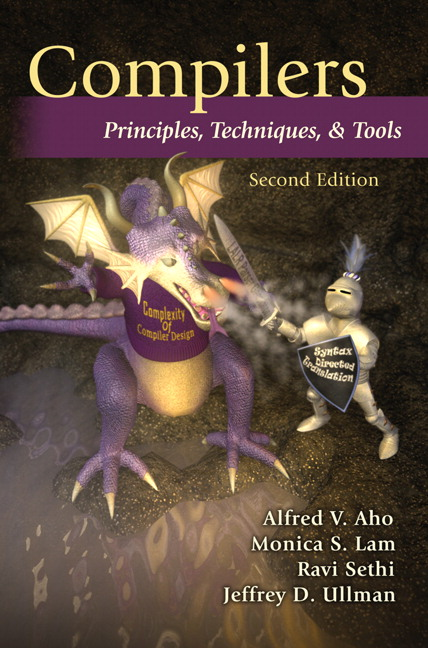
\includegraphics{dragonbook2e.jpg}}
\end{minipage}
\end{frame}


%\begin{frame}{Schedule}
%
%\textbf{Lectures:} Mondays and Wednesdays, 2:40 -- 3:55 PM
%
%833 Seeley W. Mudd Building
%
%Jan 23 -- May 6
%
%\vfill
%
%\renewcommand{\arraystretch}{1.8}
%\begin{tabular}{@{}ll}
%\textbf{Midterm Exam} & Mar 13\\
%\textbf{Final Exam} & May 6\\
%\textbf{Presentations} & May 15$^*$\\
%\textbf{Final Team project reports} & May 15\\
%\end{tabular}
%\medskip
%
%{\footnotesize $^*$ You can present before May 15.  All team members
%  must present.}
%
%\end{frame}

\begin{frame}{Prerequisites}

\textbf{COMS W3157 Advanced Programming}

\begin{itemize}

\item How to work on a large software system in a team

\item Makefiles, version control, test suites

\item Testing will be as important as coding
\end{itemize}

\textbf{COMS W3261 Computer Science Theory}

\begin{itemize}
\item Regular languages and expressions

\item Context-free grammars

\item Finite automata (NFAs and DFAs)

\end{itemize}

\end{frame}

\begin{frame}{Collaboration}

  Read the CS Department's Academic Honesty Policy:
  \url{https://www.cs.columbia.edu/education/honesty/}

Collaborate with your team on the project.

Do your homework by yourself.

\begin{itemize}
\item \textcolor{darkgreen}{OK}: Discussing lecture content, OCaml features
\item \textcolor{mRed}{Not OK}: Solving a homework problem with classmates
\item \textcolor{mRed}{Not OK}: Posting any homework questions or solutions
\end{itemize}

\alert{Don't be a cheater (e.g., copy from each other)}

\end{frame}

\part{The Team Project}

\begin{frame}{The Team Project}

Design and implement your own little language.

\textbf{Six} deliverables:

\begin{enumerate}
\item A proposal describing your language (due Feb 11)
\item A language reference manual (due Feb 27)
\item A milestone: compiling ``Hello World'' (due Apr 1)
\item A compiler for it, written in OCaml; generating LLVM
\item A final project report (due May 15)
\item A final project presentation (due May 15)
\end{enumerate}

\end{frame}

\begin{frame}{Teams}

Immediately start forming four-person teams

Each team will develop its own language

Each teach member should participate in design, coding, testing, and
documentation

\renewcommand\arraystretch{1.2}
\begin{tabular}{lp{15pc}}
\toprule
\textbf{Role} & \textbf{Responsibilities} \\
\midrule
Manager & Timely completion of deliverables \\
Language Guru & Language design \\
System Architect & Compiler architecture, \hfill\break development environment \\
Tester & Test plan, test suites \\
\bottomrule
\end{tabular}

\end{frame}

\begin{frame}{Teams}

\begin{center}
\Huge{START EARLY!}
\end{center}
\end{frame}

\begin{frame}{How Do You Work In a Team?}


  \begin{itemize}
    \itemsep=15pt
\item Address problems sooner rather than later

\emph{If you think your teammate's a flake, you're right}

\item Complain to me or your TA as early as possible

\emph{Alerting me a day before the project is due isn't helpful}

\item Not every member of a team will get the same grade

\emph{Remind your slacking teammates of this early and often}
\end{itemize}

\end{frame}

\begin{frame}{First Three Tasks}

  \begin{enumerate}
    \itemsep=15pt
\item Decide who you will work with

\emph{You'll be stuck with them for the term; choose wisely}

\item Assign a role to each member

\item Select a weekly meeting time

\emph{Harder than you might think}
\end{enumerate}

%\centerline{\includegraphics[width=1\textwidth]{when-i-die.jpg}}

\end{frame}

\begin{frame}{Project Proposal}

  \begin{itemize}
    \itemsep=15pt

\item Describe the language that you plan to implement.

\item Explain what sorts of programs are meant to be written in your language

\item Explain the parts of your language and what they do

\item Include the source code for an interesting program in your language

\item 2--4 pages
\end{itemize}

\end{frame}

\begin{frame}{Language Reference Manual}

  \begin{itemize}
    \itemsep=15pt

\item A careful definition of the syntax and semantics of your language.

\item Follow the style of the C language reference manual (Appendix A of
Kernighan and Ritchie, \emph{The C Programming Langauge}; see the
class website).

\end{itemize}

\centerline{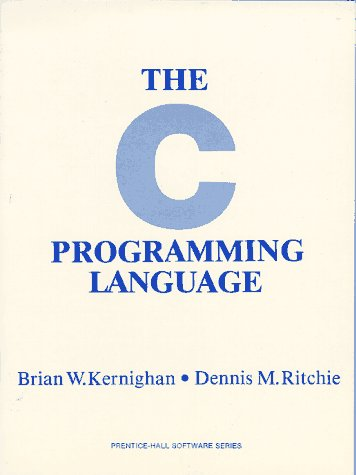
\includegraphics[width=0.3\textwidth]{kandr-first-edition.jpg}}

\end{frame}

\begin{frame}{Final Report Sections}
\renewcommand\arraystretch{1.2}
\begin{tabular}{ll}
\toprule
\textbf{Section} & \textbf{Author} \\
\midrule
Introduction & Team \\
Tutorial & Team \\
Reference Manual & Team \\
Project Plan & Manager \\
Language Evolution & Language Guru \\
Translator Architecture & System Architect \\
Test plan and scripts & Tester \\
Conclusions & Team \\
Full Code Listing & Team \\
\bottomrule
\end{tabular}

\end{frame}

\begin{frame}{Project Due Dates}

\renewcommand{\arraystretch}{2}
\begin{tabular}{@{}ll@{}}
Proposal & Feb 11 \alert{soon} \\
Language Reference Manual and Parser & Feb 27 \\
Hello World Demo & Apr 1 \\
Final Report and Presentation  & May 15 \\
\end{tabular}

\end{frame}

\begin{frame}{Design a language?}

A domain-specific language: awk or PHP, not Java or C++.

\medskip

\alert{Examples from earlier terms:}

  \begin{itemize}
    \itemsep=15pt

\item Matlab-like array manipulation language

\item Geometric figure drawing language

\item Music manipulation language

\item Mathematical function manipulator

\item Simple scripting language (\`a l\'a Tcl)
\end{itemize}

\end{frame}

\begin{frame}{Three Common Mistakes to Avoid}

Configuration File Syndrome

\begin{itemize}

\item Your language should have more than just nouns
  
\item Must be able to express \emph{algorithms}, not just data

\end{itemize}

Standard Library Syndrome

\begin{itemize}

\item Good languages enable you to \emph{build} abstractions, \break not just
  \emph{provide} them

\item Write your standard library in your language

\item Aim for Legos, not Microsoft Word
\end{itemize}

C-to-C Translator Syndrome
\begin{itemize}
\item Your compiler's output should not look like its input
\end{itemize}

\end{frame}

\begin{frame}{What I'm Looking For}

Your language must be able to express different algorithms
\begin{itemize}
\item Avoid Configuration File Syndrome.  Most languages should be
  able to express, e.g., the GCD algorithm.
\end{itemize}

Your language should consist of pieces that can mix freely

\begin{itemize}
\item Avoid Standard Library Syndrome.  For anything you provide in
  the language, ask yourself whether you can express it using other
  primitives in your language.
\end{itemize}

Your compiler must generate LLVM code

\begin{itemize}
\item Compilers should lower the level of abstraction; LLVM provides a
  machine-independent, low-level IR.
  
\item Robust, widespread ``collection of modular and reusable
compiler and toolchain technologies.''
\end{itemize}

\end{frame}


\part{Great Moments in Evolution}

\begin{frame}[fragile]{Assembly Language}

  \begin{columns}
    \begin{column}[t]{0.3\textwidth}

      \alert{Before: numbers}

      \medskip

\begin{shadedverbatim}
55    
89E5  
8B4508
8B550C
39D0  
740D
39D0  
7E08  
29D0  
39D0  
75F6  
C9    
C3    
29C2  
EBF6
\end{shadedverbatim}   
    
    \end{column}
    \begin{column}[t]{0.6\textwidth}

      \alert{After: Symbols}

      \medskip

\begin{shadedverbatim}
gcd: pushl %ebp
     movl  %esp, %ebp
     movl  8(%ebp), %eax
     movl  12(%ebp), %edx
     cmpl  %edx, %eax
     je    .L9
.L7: cmpl  %edx, %eax
     jle   .L5
     subl  %edx, %eax
.L2: cmpl  %edx, %eax
     jne   .L7
.L9: leave
     ret
.L5: subl  %eax, %edx
     jmp   .L2
\end{shadedverbatim}

    \end{column}
  \end{columns}

\end{frame}

\begin{frame}[fragile]{FORTRAN}

  \begin{columns}
    \begin{column}[t]{0.5\textwidth}
      
  \alert{Before}

  \medskip

\begin{shadedverbatim}
gcd: pushl %ebp
     movl  %esp, %ebp
     movl  8(%ebp), %eax
     movl  12(%ebp), %edx
     cmpl  %edx, %eax
     je    .L9
.L7: cmpl  %edx, %eax
     jle   .L5
     subl  %edx, %eax
.L2: cmpl  %edx, %eax
     jne   .L7
.L9: leave
     ret
.L5: subl  %eax, %edx
     jmp   .L2
\end{shadedverbatim}

    \end{column}
\begin{column}[t]{0.5\textwidth}

  \alert{After: Expressions, control-flow}

  \medskip

\begin{fortran}
 10   if (a .EQ. b) goto 20
      if (a .LT. b) then
         a = a - b
      else
         b = b - a
      endif
      goto 10
 20   end
\end{fortran}

\end{column}
  \end{columns}

  \vfill
  
\begin{leftpopup}
Backus, IBM, 1956

Imperative language for science and engineering

First compiled language

Fixed format punch cards

Arithmetic expressions, If, Do, and Goto statements

Scalar and array types

Limited string support

Still common in high-performance computing

Inspired most modern languages, especially BASIC
\end{leftpopup}


\end{frame}

\begin{frame}[fragile]{COBOL}

\alert{Added type declarations, record types, file manipulation}

\begin{shadowblock}
\begin{lstlisting}[language=Cobol]
data division.
file section.
*   describe the input file
fd  employee-file-in
            label records standard
            block contains 5 records
            record contains 31 characters
            data record is employee-record-in.
01  employee-record-in.
    02  employee-name-in  pic x(20).
    02  employee-rate-in  pic 9(3)v99.
    02  employee-hours-in pic 9(3)v99.
    02  line-feed-in      pic x(1).
\end{lstlisting}
\end{shadowblock}

\begin{columns}
  \begin{column}{0.35\textwidth}
    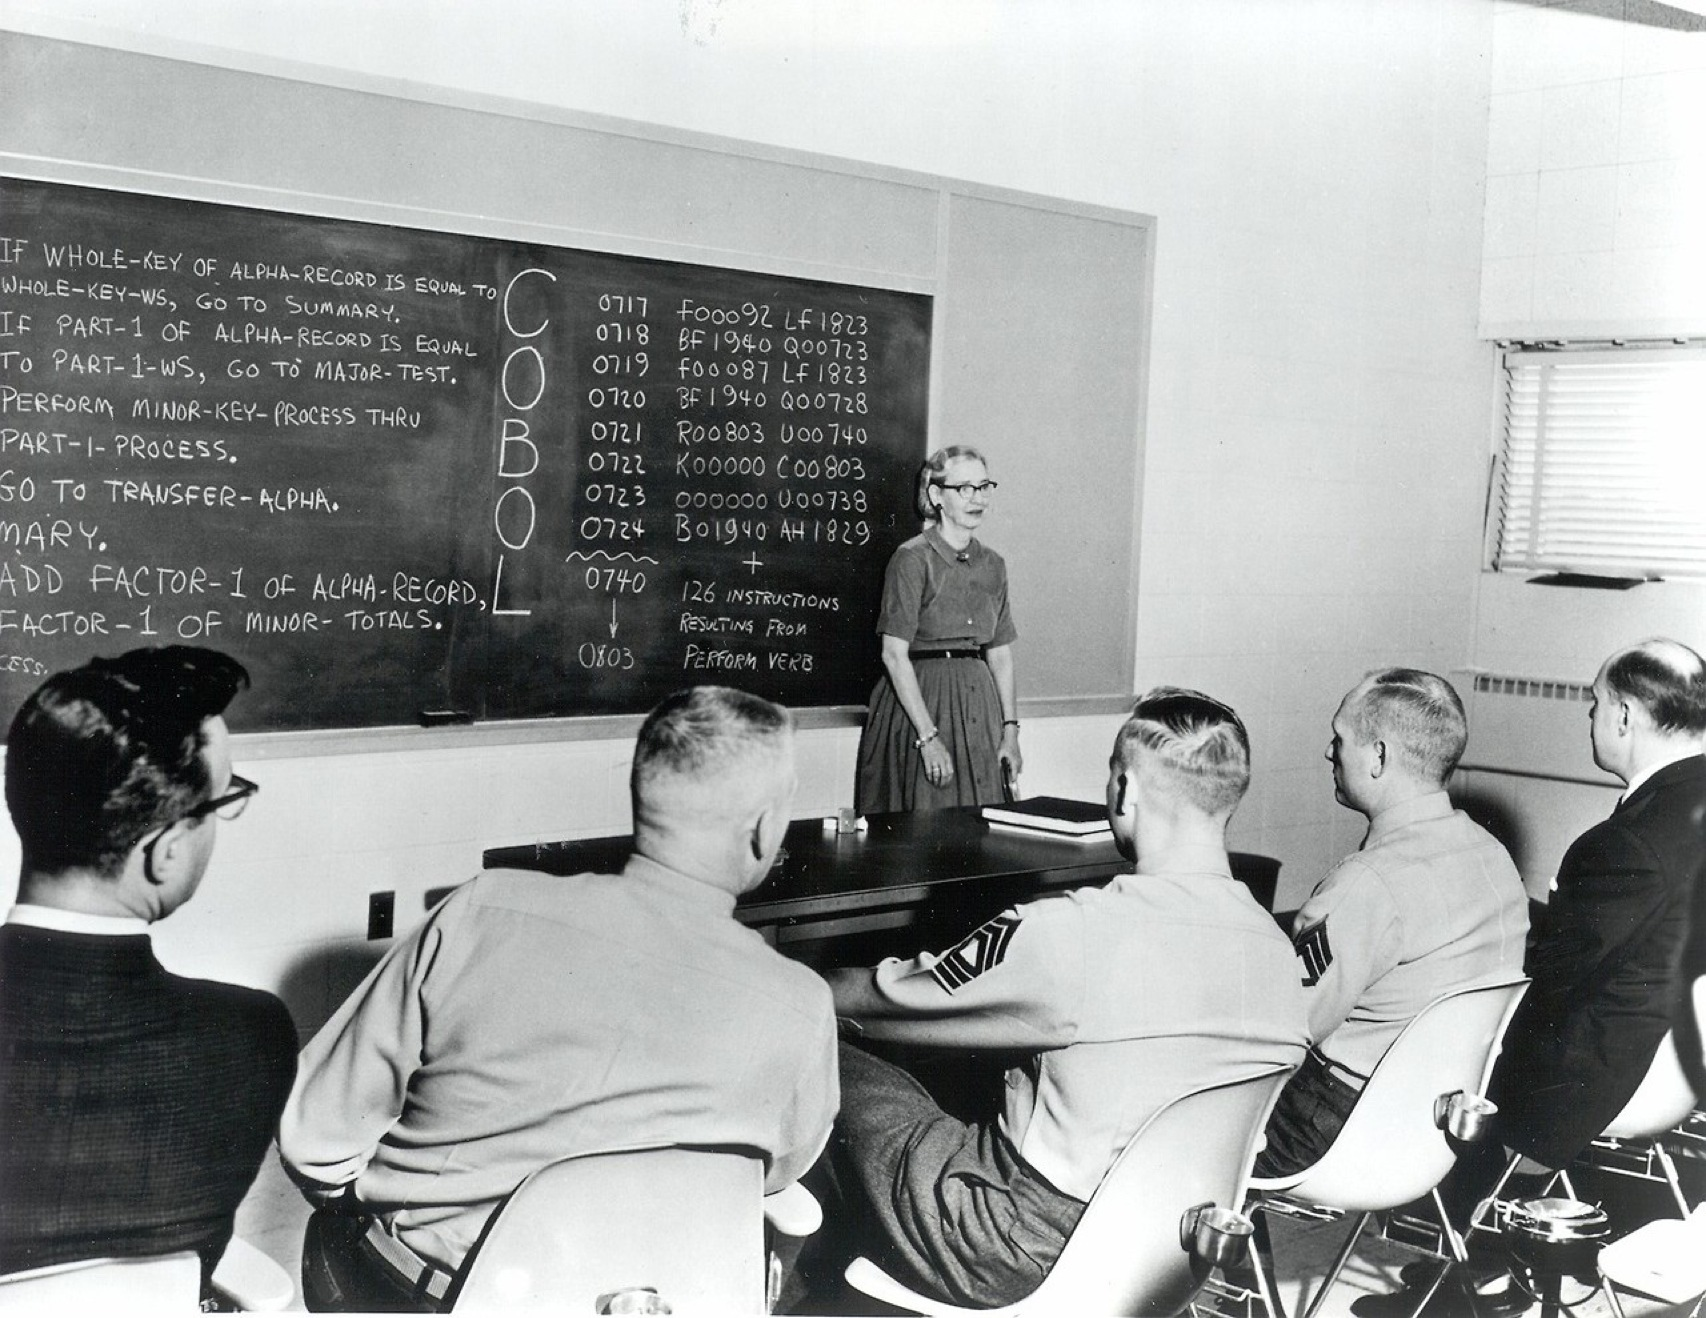
\includegraphics[width=\textwidth]{grace-cobol.jpg}
  \end{column}%
  \begin{column}{0.65\textwidth}

English-like syntax: 300 reserved words

Grace Hopper et al.

  \end{column}
\end{columns}
\end{frame}

\begin{frame}[fragile]{LISP, Scheme, Common LISP}

\alert{Functional, high-level languages}

\begin{shadowblock}
\begin{lstlisting}[language=Lisp]
(defun append (l1 l2)
  (if (null l1)
      l2
      (cons (first l1) (append (rest l1) l2))))
\end{lstlisting}
\end{shadowblock}
% $

\vspace{8\baselineskip}

\begin{rightpopup}
McCarthy, MIT, 1958

Functional: recursive, list-focused functions

Semantics from Church's Lambda Calculus

Simple, heavily parenthesized S-expression syntax

Dynamically typed

Automatic garbage collection

Originally for AI applications

Dialects: Scheme and Common Lisp
\end{rightpopup}

\end{frame}

\begin{frame}{APL}

\alert{Powerful operators, interactive, custom character set}

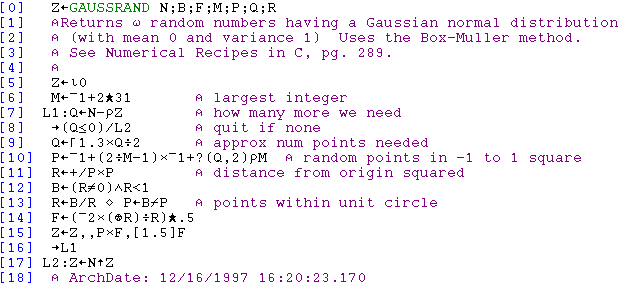
\includegraphics[width=\textwidth]{apl-program.png}

{\small ``Emoticons for Mathematicians''}

{\tiny Source: Jim Weigang,
  http://www.chilton.com/\char`\~jimw/gsrand.html

At right: Datamedia APL Keyboard}


%\vspace{4pc}

\hfill \begin{minipage}{0.4\textwidth}
\vspace{-8pc}
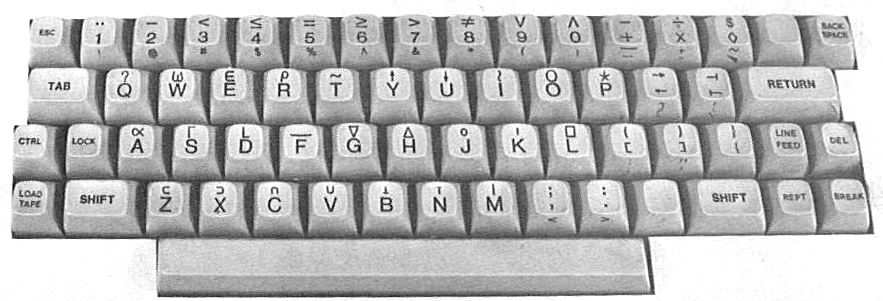
\includegraphics[width=\textwidth,clip=true,viewport=75 50 275 250]{datamedia-apl-keyboard.jpg}
\end{minipage}

\begin{rightpopup}
Iverson, IBM, 1960

Imperative, matrix-centric

E.g., perform an operation on each element of a vector

Uses own specialized character set

Concise, effectively cryptic

Primarily symbols instead of words

Dynamically typed

Odd left-to-right evaluation policy

Useful for statistics, other matrix-oriented applications
\end{rightpopup}

\end{frame}


\begin{frame}[fragile]{Algol, Pascal, Clu, Modula, Ada}

\emph{Imperative, block-structured language, formal syntax definition,
  structured programming}

\begin{shadowblock}
\begin{lstlisting}[basicstyle={\fontsize{9}{9.5}\selectfont\ttfamily},language=Algol]
PROC insert = (INT e, REF TREE t)VOID:
   # NB inserts in t as a side effect #
   IF TREE(t) IS NIL THEN
     t := HEAP NODE := (e, TREE(NIL), TREE(NIL))
   ELIF e < e OF t THEN insert(e, l OF t)
   ELIF e > e OF t THEN insert(e, r OF t)
   FI;

 PROC trav = (INT switch, TREE t, SCANNER continue,
              alternative)VOID:
   # traverse the root node and right sub-tree of t  only. #
   IF t IS NIL THEN continue(switch, alternative)
   ELIF e OF t  <=  switch THEN
         print(e OF t);
         traverse( switch, r OF t, continue, alternative)
   ELSE  # e OF t > switch #
         PROC defer = (INT sw, SCANNER alt)VOID:
               trav(sw, t, continue, alt);
         alternative(e OF t, defer)
   FI;
\end{lstlisting}
\end{shadowblock}

\tiny Algol-68, source http://www.csse.monash.edu.au/\char`\~lloyd/tildeProgLang/Algol68/treemerge.a68

\end{frame}

\begin{frame}[fragile]{SNOBOL, Icon}

\alert{String-processing languages}

\begin{shadedverbatim}
   LETTER  =  'ABCDEFGHIJKLMNOPQRSTUVWXYZ$#@'
   SP.CH   =  "+-,=.*()'/& "
   SCOTA  =  SP.CH
   SCOTA   '&'  =
   Q  =  "'"
   QLIT  =  Q  FENCE  BREAK(Q)  Q
   ELEM  =  QLIT | 'L' Q | ANY(SCOTA) | BREAK(SCOTA) | REM
   F3  =  ARBNO(ELEM FENCE)
   B  =  (SPAN(' ') | RPOS(0))  FENCE
   F1  =  BREAK(' ')  |  REM
   F2  =  F1
   CAOP  =  ('LCL'  |  'SET')  ANY('ABC')  |
+  'AIF'  |  'AGO'  |  'ACTR'  |  'ANOP'
   ATTR  =  ANY('TLSIKN')
   ELEMC  =  '(' FENCE *F3C ')'  |  ATTR Q  |  ELEM
   F3C    =  ARBNO(ELEMC  FENCE)
   ASM360  =  F1 . NAME  B
+  ( CAOP . OPERATION  B  F3C . OPERAND  |
+  F2 . OPERATION    B  F3 . OPERAND)
+  B    REM . COMMENT
\end{shadedverbatim}

\tiny SNOBOL: Parse IBM 360 assembly.  From Gimpel's book, http://www.snobol4.org/

\end{frame}

\begin{frame}[fragile]{BASIC}

\alert{Programming for the masses}

\begin{shadowblock}
\lstset{language=[Visual]Basic}
\begin{lstlisting}
10 PRINT "GUESS A NUMBER BETWEEN ONE AND TEN"
20 INPUT A$
30 IF A$ <> "5" THEN GOTO 60
40 PRINT "GOOD JOB, YOU GUESSED IT"
50 GOTO 100
60 PRINT "YOU ARE WRONG. TRY AGAIN"
70 GOTO 10
100 END
\end{lstlisting}
\end{shadowblock}
% $

\parbox[b]{0.55\textwidth}{\raggedright
Invented at Dartmouth by \\John George Kemeny and Thomas
Eugene Kurtz.  Started the whole Bill Gates/ Microsoft thing.  
}%
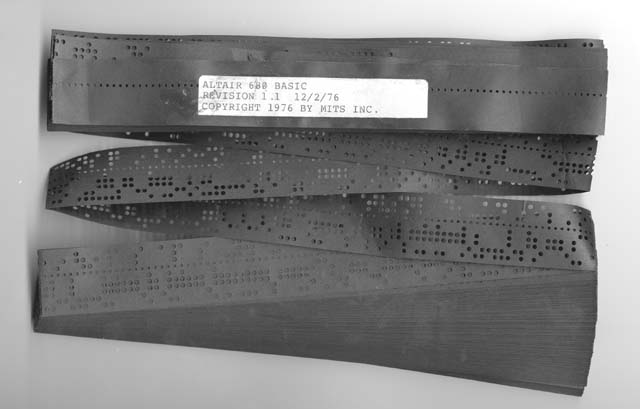
\includegraphics[width=0.45\textwidth]{altair-basic-papertape.jpg}

\end{frame}

\begin{frame}[fragile]{Simula, Smalltalk, C++, Java, C\#}

\alert{The object-oriented philosophy}

\begin{shadedverbatim}
class Shape(x, y); integer x; integer y;
virtual: procedure draw;
begin
   comment -- get the x & y coordinates --;
   integer procedure getX;
      getX := x;
   integer procedure getY;
      getY := y;

   comment -- set the x & y coordinates --;
   integer procedure setX(newx); integer newx;
      x := newx;
   integer procedure setY(newy); integer newy;
      y := newy;
end Shape;
\end{shadedverbatim}
\end{frame}

\begin{frame}[fragile]{99 Bottles of Beer in Java}

\begin{java}
class Bottles {
  public static void main(String args[]) {
    String s = "s";
    for (int beers=99; beers>-1;) {
      System.out.print(beers+" bottle"+s+" of beer on the wall, ");
      System.out.println(beers + " bottle" + s + " of beer, ");
      if (beers==0) {
        System.out.print("Go to the store, buy some more, ");
        System.out.println("99 bottles of beer on the wall.\n");
        System.exit(0);
      } else
        System.out.print("Take one down, pass it around, ");
      s = (--beers == 1)?"":"s";
      System.out.println(beers+" bottle"+s+" of beer on the wall.\n");
    }
  }
}
\end{java}

\begin{rightpopup}
Gosling et al., Sun, 1991

Imperative, object-oriented, threaded

Based on C++, C, Algol, etc.

Statically typed

Automatic garbage collection

Architecturally neutral

Defined on a virtual machine (Java Bytecode)
\end{rightpopup}

\footnotesize 
Sean Russell,
 \url{http://www.99-bottles-of-beer.net/language-java-4.html}

\end{frame}

\begin{frame}[fragile]{C}

\alert{Efficiency for systems programming}

\begin{C}
int gcd(int a, int b)
{
  while (a != b) {
    if (a > b) a -= b;
    else b -= a;
  }
  return a;
}
\end{C}

\vfill

\begin{rightpopup}
Dennis Ritchie, Bell Labs, 1969

Procedural, imperative

Based on Algol, BCPL

Statically typed; liberal conversion policies

Harmonizes with processor architecture

For systems programming: unsafe by design

Remains language of choice for operating systems
\end{rightpopup}

\end{frame}


\begin{frame}[fragile]{ML, Miranda, Haskell}

\alert{Functional languages with types and syntax}

\begin{shadowblock}
\small\baselineskip=5pt
\begin{lstlisting}[language=ML]
structure RevStack = struct
  type  'a stack =  'a list
  exception Empty
  val empty = []
  fun isEmpty (s:'a stack):bool =
    (case s
       of [] => true
        | _ => false)
  fun top (s:'a stack): =
    (case s
       of [] => raise Empty
        | x::xs => x)
  fun pop (s:'a stack):'a stack =
    (case s
        of [] => raise Empty
         | x::xs => xs)
  fun push (s:'a stack,x: 'a):'a stack = x::s
  fun rev (s:'a stack):'a stack = rev (s)
end
\end{lstlisting}
\end{shadowblock}

\end{frame}


\begin{frame}[fragile]{99 Bottles of Beer in Haskell}

\begin{haskell}
bottles :: Int -> String
bottles n
  | n == 0 = "no more bottles"
  | n == 1 = "1 bottle"
  | n >  1 = show n ++ " bottles"

verse :: Int -> String
verse n
  | n == 0 = "No more bottles of beer on the wall, "
             ++ "no more bottles of beer.\n"
             ++ "Go to the store and buy some more, "
             ++ "99 bottles of beer on the wall."
  | n > 0  = bottles n ++ " of beer on the wall, "
             ++ bottles n
             ++ " of beer.\n"
             ++ "Take one down and pass it around, "
             ++ bottles (n-1) ++ " of beer on the wall.\n"

main      = mapM (putStrLn . verse) [99,98..0]
\end{haskell}

\begin{rightpopup}
Peyton Jones et al., 1990

Functional

Pure: no side-effects

Lazy: computation only on demand; infinite data structures

Statically typed; types inferred

Algebraic data types, pattern matching, lists, strings

Great for compilers, domain-specific languages, type system research

Related to ML, OCaml
\end{rightpopup}

\footnotesize Simon Johansson,
\url{http://www.99-bottles-of-beer.net/language-haskell-1613.html}
\end{frame}

\begin{frame}[fragile]{sh, awk, perl, tcl, python, php}

\alert{Scripting languages: glue for binding the universe together}

\begin{shadowblock}
\begin{lstlisting}[language=sh]
class() {
  classname=`echo "$1" | sed -n '1 s/ *:.*$//p'`
  parent=`echo "$1" | sed -n '1 s/^.*: *//p'`
  hppbody=`echo "$1" | sed -n '2,$p'`

  forwarddefs="$forwarddefs
  class $classname;"

  if (echo $hppbody | grep -q "$classname()"); then
    defaultconstructor=
  else
    defaultconstructor="$classname() {}"
  fi
}
\end{lstlisting}
\end{shadowblock}

\end{frame}

\begin{frame}[fragile]{99 Bottles of Beer in AWK}

\begin{awk}
BEGIN { 
   for(i = 99; i >= 0; i--) {
      print ubottle(i), "on the wall,", lbottle(i) "."
      print action(i), lbottle(inext(i)), "on the wall."
      print
   }
}
function ubottle(n) {
   return sprintf("%s bottle%s of beer", n?n:"No more", n-1?"s":"")
}
function lbottle(n) {
   return sprintf("%s bottle%s of beer", n?n:"no more", n-1?"s":"")
}
function action(n) {
   return sprintf("%s", n ? "Take one down and pass it around," : \
                            "Go to the store and buy some more,")
}
function inext(n) {
   return n ? n - 1 : 99
}
\end{awk}

\begin{rightpopup}
Aho, Weinberger, and Kernighan, Bell Labs, 1977

Interpreted domain-specific scripting language for text processing

Pattern-action statements matched against input lines

C-inspired syntax

Automatic garbage collection
\end{rightpopup}

\footnotesize OsamuAoki,
\url{http://www.99-bottles-of-beer.net/language-awk-1623.html}

\end{frame}

\begin{frame}[fragile]{AWK (bottled version)}

\begin{columns}
  \begin{column}[b]{0.5\textwidth}

    \footnotesize Wilhelm Weske,
\url{http://www.99-bottles-of-beer.net/language-awk-1910.html}

\end{column}
\begin{column}[b]{0.5\textwidth}
\vbox to 0.8\textheight{
\vss
\begin{awk}
        BEGIN{
       split( \
       "no mo"\
       "rexxN"\
       "o mor"\
       "exsxx"\
       "Take "\
      "one dow"\
     "n and pas"\
    "s it around"\
   ", xGo to the "\
  "store and buy s"\
  "ome more, x bot"\
  "tlex of beerx o"\
  "n the wall" , s,\
  "x"); for( i=99 ;\
  i>=0; i--){ s[0]=\
  s[2] = i ; print \
  s[2 + !(i) ] s[8]\
  s[4+ !(i-1)] s[9]\
  s[10]", " s[!(i)]\
  s[8] s[4+ !(i-1)]\
  s[9]".";i?s[0]--:\
  s[0] = 99; print \
  s[6+!i]s[!(s[0])]\
  s[8] s[4 +!(i-2)]\
  s[9]s[10] ".\n";}}
\end{awk}
\vss
}
\end{column}
\end{columns}

\end{frame}

\begin{frame}[fragile]{99 Bottles of Beer in Python}

\begin{python}
for quant in range(99, 0, -1):
   if quant > 1:
      print quant, "bottles of beer on the wall,", \
            quant, "bottles of beer."
      if quant > 2:
         suffix = str(quant - 1) + " bottles of beer on the wall."
      else:
         suffix = "1 bottle of beer on the wall."
   elif quant == 1:
      print "1 bottle of beer on the wall, 1 bottle of beer."
      suffix = "no more beer on the wall!"
   print "Take one down, pass it around,", suffix
   print ""
\end{python}

\begin{rightpopup}
Guido van Rossum, 1989

Object-oriented, imperative

General-purpose scripting language

Indentation indicates grouping

Dynamically typed

Automatic garbage collection
\end{rightpopup}

\footnotesize Gerold Penz, \\
\url{http://www.99-bottles-of-beer.net/language-python-808.html}

\end{frame}


\begin{frame}[fragile]{99 Bottles of Beer in FORTH}

\begin{forth}
: .bottles ( n -- n-1 )
   dup 1 = IF  ." One bottle of beer on the wall," CR
               ." One bottle of beer," CR
               ." Take it down," 
   ELSE  dup . ." bottles of beer on the wall," CR
         dup . ." bottles of beer," CR
         ." Take one down," 
   THEN
   CR
   ." Pass it around," CR
   1-
   ?dup IF  dup 1 = IF  ." One bottle of beer on the wall;" 
            ELSE  dup . ." bottles of beer on the wall;" 
            THEN
        ELSE  ." No more bottles of beer on the wall." 
   THEN
   CR
;
: nbottles ( n -- )
  BEGIN  .bottles  ?dup NOT UNTIL ;

99 nbottles
\end{forth}

\begin{rightpopup}
Moore, NRAO, 1973

Stack-based imperative language

Trivial, RPN-inspired grammar

Easily becomes cryptic

Untyped

Low-level, very lightweight

Highly extensible: easy to make programs compile themselves

Used in some firmware boot systems (Apple, IBM, Sun)

Inspired the PostScript language for laser printers
\end{rightpopup}

\footnotesize Dan Reish, \url{http://www.99-bottles-of-beer.net/language-forth-263.html}

\end{frame}

\begin{frame}<2>{The Whitespace Language}

\vspace{0.8\textheight}

\begin{rightpopup}
Edwin Brady and Chris Morris, April 1st, 2003

Imperative, stack-based language

Space, Tab, and Line Feed characters only

Number literals in binary: Space=0, Tab=1, LF=end

Less-than-programmer-friendly syntax; reduces toner consumption
\end{rightpopup}
\footnotesize
Andrew Kemp, \url{http://compsoc.dur.ac.uk/whitespace/}

\end{frame}

\begin{frame}[fragile]{VisiCalc, Lotus 1-2-3, Excel}

\alert{The spreadsheet style of programming}

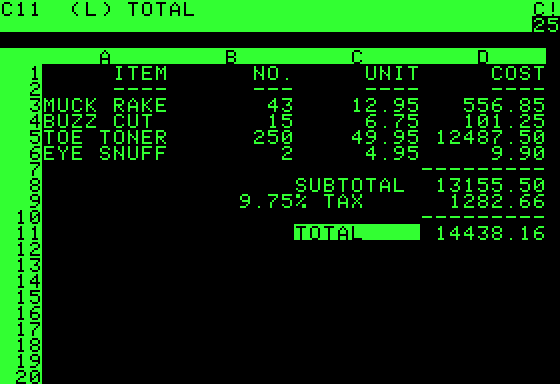
\includegraphics[width=0.8\textwidth]{visicalc.png}

Visicalc on the Apple II, c. 1979

\end{frame}

\begin{frame}[fragile]{SQL}

\alert{Database queries}

\begin{shadowblock}
\begin{lstlisting}[language=SQL]
CREATE TABLE shirt (
    id SMALLINT UNSIGNED NOT NULL AUTO_INCREMENT,
    style ENUM('t-shirt', 'polo', 'dress') NOT NULL,
    color ENUM('red', 'blue', 'white', 'black') NOT NULL,
    owner SMALLINT UNSIGNED NOT NULL
          REFERENCES person(id),
    PRIMARY KEY (id)
);

INSERT INTO shirt VALUES
(NULL, 'polo', 'blue', LAST_INSERT_ID()),
(NULL, 'dress', 'white', LAST_INSERT_ID()),
(NULL, 't-shirt', 'blue', LAST_INSERT_ID());
\end{lstlisting}
\end{shadowblock}

\begin{rightpopup}
Chamberlin and Boyce, IBM, 1974

Declarative language for databases

Semantics based on the relational model

Queries on tables: select with predicates, joining, aggregating

Database query optimization: declaration to procedure
\end{rightpopup}

\end{frame}

\begin{frame}[fragile]{Prolog}

\alert{Logic Language}

\begin{shadowblock}
\begin{lstlisting}[language=Prolog]
witch(X)  <= burns(X), female(X).
burns(X)  <= wooden(X).
wooden(X) <= floats(X).
floats(X) <= sameweight(duck, X).

female(girl).          {by observation}
sameweight(duck,girl). {by experiment }

? witch(girl).
\end{lstlisting}
\end{shadowblock}

\vspace{-1pc}

\hfill

\includegraphics[width=0.4\textwidth]{monty-python-holy-grail-witch.jpg}

\begin{rightpopup}
Alain Colmerauer et al., 1972

Logic programming language

Programs are relations: facts and rules

Program execution consists of trying to satisfy queries

Designed for natural language processing, expert systems, and theorem proving
\end{rightpopup}


\end{frame}

\end{document}

% Local Variables:
% compile-command: "make intro.pdf"
% End:
